%        File: report.tex
%     Created: Fri Mar 27 08:00 AM 2015 G
% Last Change: Fri Mar 27 08:00 AM 2015 G

   
% \documentclass[a4paper]{article}

%%% Start of User defined preamble:

\documentclass[a4paper, 11pt]{article}
\usepackage[english]{babel}
\usepackage[T1]{fontenc} % For å bruke æøå
\usepackage[utf8]{inputenc}
\usepackage{amsmath}
\usepackage{amssymb}
\usepackage{graphicx}
\usepackage{hyperref}
\usepackage{cite}

\title{Monte Carlo Simulations \\
Report: Problem Sheet 5 \\ A real-world application of MCMC}
\author{Kristian Bjørke}
\date{09.04.2015}

%%% End of User defined preamble:

% Have to fix up references!!!
\bibliographystyle{abbrv}

\begin{document}
\maketitle

\begin{abstract}
  In this project we have used a Markov Chain Monte Carlo(MCMC) method to
  decrypt a substitution cipher message, using statistical properties 
  of the english language. By obtaining these statistical properties 
  from analysing ``War and Peace'' by Lev Tolstoy and using a MCMC 
  computer program written in R we have  decoded a message starting with 
  ``DK PDUJVDO KSOSIUXAP DIUK  KAOSOQ BQ UMS HVSKSVCDUXAP AR$\dots$''. 
  We found the decoded message to be a paragraph taken from ``On the 
  Origin of Species'' by Charles Darwin starting with ``AS NATURAL 
  SELECTION ACTS SOLELY BY THE PRESERVATION OF$\dots$''.
\end{abstract}


\section{Introduction}

The purpose of this project is to use a Markov Chain Monte Carlo(MCMC) 
process to decrypt a encrypted text. We will focus on text that has been 
encrypted by the substitution cipher, which means that each letter in 
the alphabet has been replaced by another letter in the alphabet.

Each student have been given such a encrypted substitution cipher text.
Following is the one that I was given:

DK PDUJVDO KSOSIUXAP DIUK KAOSOQ BQ UMS HVSKSVCDUXAP AR
HVARXUDBOS ZANXRXIDUXAPK, SDIM PSF RAVZ FXOO USPN XP D RJOOQ-
KUAITSN IAJPUVQ UA UDTS UMS HODIS AR, DPN RXPDOOQ UA SEUSVZXPDUS, XUK
AFP OSKK XZHVACSN HDVSPU-RAVZ DPN AUMSV OSKK-RDCAJVSN RAVZK FXUM
FMXIM XU IAZSK XPUA IAZHSUXUXAP.

The papers \cite{Diaconis}, \cite{Chen} and \cite{Kocmanek} have been helpfull
while creating the R program for the Markov Chain Monte Carlo process of
decoding. While \cite{Landgraf} was helpfull to make a program that could
aquire the nececary statistics about english text needed for the decryption.

First we will outline the Markov Chain Monte Carlo decryption method that
we will use to decrypt the substitution cipher text. Then we will decribe how
we will obtain the nececary statistics about english texts by analysing the
text ``War and Peace'' by Lev Tolstoy.

After this we will present some results from applying the MCMC method to
our given text and a example text, and discuss the quality of the results.
Last we will finish with a conclusion where we sum up our findings.

At the end of the text we will include listings of the R code that was used
in this project. The source code, results and other files relevant for this
project are also available from the following GitHub repository:

\href{http://github.com/kbjorke/MCS-Problem-5}{http://github.com/kbjorke/MCS-Problem-5}


\section{Markov Chain Monte Carlo decryption method}

The MCMC method that I will be using i based mainly on \cite{Kocmanek}.

We will view the substitution ciphering as applying a function $g$ on the
message, which we call the plaintext. This function maps the text from the
decoded space into the encrypted space by returning a replacement character
for each character.

We are given an encrypted text, called the ciphertext, which has been 
encrypted by a unknown cipher function $g$, and we want to find the 
inverse function $f = g^{-1}$ that maps the ciphertext back to the plaintext,
which contains the decoded message.

We assume that the encrypted text we are given is based on a plaintext 
written in english. Characteristic for english texts are the transition 
probability matrix $M(X,Y)$ and the character probabilities $p(X)$, where
$X$ and $Y$ are any characters.

The probability matrix $M(X,Y)$ gives us the probability that the character
$Y$ will follow the character $X$ in an arbitrary english text. The
character probabilites $p(X)$ gives the probability of $X$ beein a randomly
selected character in an english text. A better way is to call $p(X)$ the
relative frequency of the character $X$ appearing in an english text.

We will attempt to find the decryption key $f$ by solving it as a maximum
likelihood problem. For this purpose we define the score function $\pi(f)$ 
for a given key $f$:

\begin{equation}
  \pi(f) = \lambda_1 \sum_{i=1}^{N} p(f(s_i)) + 
  \lambda_2 \sum_{i=1}^{N-1} M(f(s_i),f(s_{i+1}))
  \label{eq:ScoreFunc}
\end{equation}

, where $s_1,s_2,\dots,s_N$ are the consecutive characters in the ciphertext
and $N$ is the length of the ciphertext. The parameters $\lambda_1$ and 
$\lambda_2$ are weights that determine if we want to emphasize the
transition probabilities or the character probabilities. We have the conditions
$\lambda_1 + \lambda_2 = 1$ and $\lambda_1, \lambda_2 \geq 0$.

We will use a Markov Chain Monte Carlo process to find the decryption key
$f$ that maximize the score function $\pi(f)$.

To choose an initial decryption key to start the Markov Chain I suggest to
find the relative frequencies of the characters in the ciphertext, compare 
these with the relative frequencies in english texts. Then assign the most
frequent character in the ciphertext to the most frequent in english texts, 
the second most frequent with the second most frequent and so on, untill
we have an initial decryption key.

Then start the Markov Chain by repeating the following steps, and denote
$t$ as the iteration number:

1. Create a new key $f_{t+1}$, where we only swap two characters of 
the current key $f_t$.

2. Calculate the acceptance ratio $a_t$ defined as
\[
  a_t = \left( \frac{\pi(f_{t+1})}{f_{t}} \right)^p
\]
, where $p$ is the scaling parameter.

3. Draw a random uniform distributed number $u_t$ in the range [0,1].

4. If the acceptance ratio is larger then the random number, $a_t \geq u_t$,
we accept the new key and discard the current key, otherwise we reject
the new key and keep the current key.

The scaling parameter $p$ is used to adjust the acceptance ratio, so that
we can avoid a local maximum or avoid to much variations around a maximum.

\section{English language properties}

In order to use the MCMC decryption methods we need to find the transition
probability matrix $M(X,Y)$ and the character probabilities $p(X)$ for
english texts. In \cite{Landgraf} there is presented a way to obtain this by
analysing a sufficiently long english text. The length of the text is
important, because it make it statistically representative for a general
english text. 

The text we will use for this analysis is the english translation of 
"War and Peace" by Lev Tolstoy, which contains about 3.1 million characters. 
This is the same text as used in \cite{Landgraf}. The text can be downloaded
from Project Gutenberg [INSERT LINK] in .txt format, which is convenient for
the analysis.

The analysis was done by first formating the text so that only letters from
the english alphabeth A-Z and whitespaces remained. Non-english letters was
replaces by corresponding english letters. All other symbols was replaces by
whitespaces.

Then we used a R script to loop through all the characters of the text
and store the frequency of each characters `` '', ``A'', ``B'', 
$\dots$, ``Z'' and also the frequency of the ordered pair of two 
characters ``XY''. At the end we normalized each row of the matrix $M(X,Y)$
and the function $p(X)$ to 1.

\begin{figure}[h!]
  \centering
  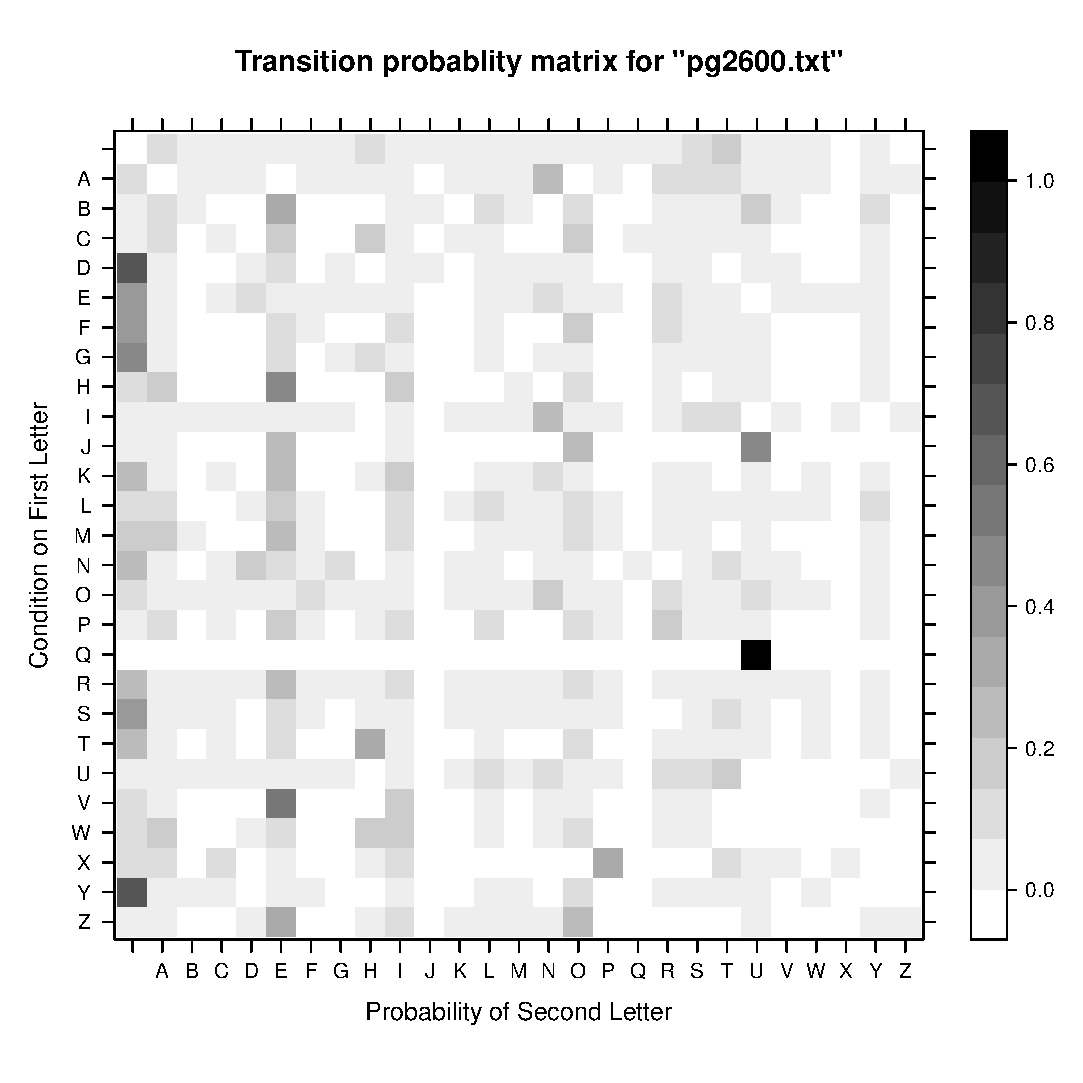
\includegraphics[width=0.6\textwidth]{transprob_matrix-pg2600-.eps}
  \caption{Transition probability matrix $M(X,Y)$ based on the text
    ``War and Peace'' by Lev Tolstoy. For comparison see \cite{Landgraf}.}
  \label{fig:TransProbMat}
\end{figure}

\begin{figure}[h!]
  \centering
  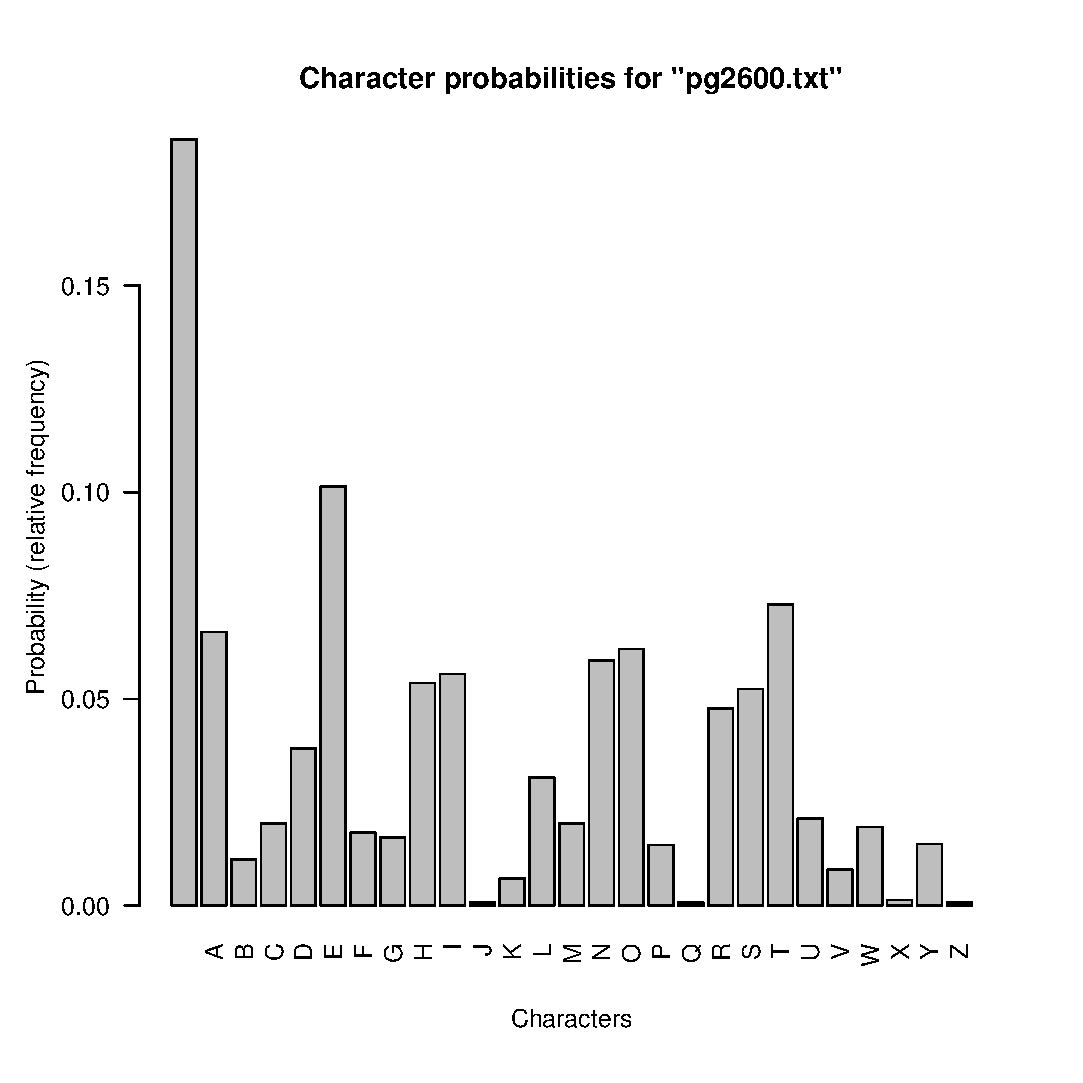
\includegraphics[width=0.6\textwidth]{char_prob-pg2600-.eps}
  \caption{Character probabilities $p(X)$ based on the text
  ``War and Peace'' by Lev Tolstoy. For comparison see [WIKI LINK]}
  \label{fig:CharProb}
\end{figure}

The result from this analysis of ``War and Peace'' by Lev Tolstoy can be
seen in the 

\section{Results and discussion}

\section{Conclusion}

\bibliography{references}

\section{Code Listings}



\end{document}


